\begin{figure}[h] 
\centering 
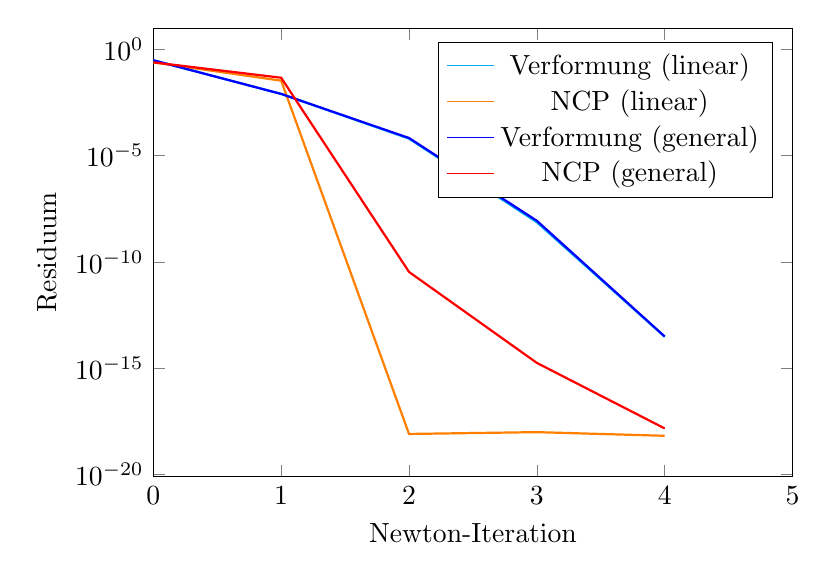
\begin{tikzpicture}[every plot/.append style={thick}] 
\begin{axis}[ 
label style={font=\normalsize}, 
xlabel={Newton-Iteration}, 
ylabel={Residuum}, 
xmin=0, xmax=5, 
ymode=log, 
ymin=0, ymax=10, 
width=0.8\textwidth, 
height=0.6\textwidth, 
legend pos=north east, 
legend style={cells={align=left}}, 
grid style=dashed, 
] 
\addplot[ 
color=cyan, 
] 
coordinates { 
(0, 3.11e-01)(1, 8.06e-03)(2, 6.34e-05)(3, 7.34e-09)(4, 2.97e-14)}; 
\addlegendentry{Verformung (linear)} 
\addplot[ 
color=orange, 
] 
coordinates { 
(0, 2.47e-01)(1, 3.40e-02)(2, 7.91e-19)(3, 9.64e-19)(4, 6.48e-19)}; 
\addlegendentry{NCP (linear)} 
\addplot[ 
color=blue, 
] 
coordinates { 
(0, 3.11e-01)(1, 8.08e-03)(2, 6.79e-05)(3, 8.60e-09)(4, 3.07e-14)}; 
\addlegendentry{Verformung (general)} 
\addplot[ 
color=red, 
] 
coordinates { 
(0, 2.47e-01)(1, 4.67e-02)(2, 3.36e-11)(3, 1.75e-15)(4, 1.44e-18)}; 
\addlegendentry{NCP (general)} 
\end{axis} 
\end{tikzpicture} 
\caption{Residuen des Stoffgesetzes 'St.Venant' mit Hinderniss 'Parabel' und 8450 Freiheitsgraden für die Verschiebung.} 
\label{fiq:St.Venant_Parabel_level5} 
\end{figure} 
